\documentclass{article} % For LaTeX2e
\usepackage{report,times}
\usepackage{hyperref}
\usepackage{url}
\usepackage{biblatex}
\usepackage{amsmath}
\usepackage{graphicx}
\usepackage{algorithmic}
\usepackage{algorithm}
\usepackage{amsfonts}
\usepackage{pgfplots}
\usepackage{pgfplotstable}
\pgfplotsset{compat = 1.17}
\graphicspath{{../figures/}}
\addbibresource{references.bib}
\pgfplotstableread[col sep=comma]{../results/FashionMNIST0.5.csv}\resultsa
\pgfplotstableread[col sep=comma]{../results/FashionMNIST0.6.csv}\resultsb
\pgfplotstableread[col sep=comma]{../results/CIFAR.csv}\resultsc
%\documentstyle[nips14submit_09,times,art10]{article} % For LaTeX 2.09


\title{Assignment 2}
\author{
  John Hu (500395897, zehu4485)\\
  Implemented classifiers\\
  Wrote most of report
  \and
  Nicholas Grasevski (500710654, ngra5777)\\
  Implemented transition matrix estimation\\
  Wrote experiment part of report
  \and
  Tutor: Yu Yao
}





\newcommand{\fix}{\marginpar{FIX}}
\newcommand{\new}{\marginpar{NEW}}

\nipsfinalcopy % Uncomment for camera-ready version

\begin{document}


\maketitle

\begin{abstract}
In this report we explore the effectiveness of robust techniques on noisy labeled datasets. Using a transition matrix that is estimated by anchor points we can improve the accuracy of a wide range of classifiers. The classifiers tested includes neural networks (ResNet, EfficientNet and LeNet) and black box classifiers (Logistic Regression and LightGBM). All classifiers are implemented on Fashion MINIST 0.5, Fashion MINIST 0.6 and CIFAR datasets. The neural networks perform well on more complex CIFAR dataset with LeNet having the highest accuracy. The black box classifiers are able to achieve similar accuracy in simpler datasets, however accuracies are poor on the CIFAR dataset.
\end{abstract}

\section{Introduction}
The rapid advancement of technology provides us with access to huge amount of data. However not all the data are clean and useable, some of them contain undesired noise which will undermine the accuracy of a classifier. In this report we explore the usage of estimating transition matrix to reduce or even eliminate label noise, hence improve the performance of classifier. Classifiers that will be used and compared are LightGBM, (multinomial) logistic regression, ResNet, EfficientNet, LeNet, and additionally some basic 1-layer and 3-layer neural networks.

\section{Related work}
There are two main elements to the label denoising approach taken in this report: the underlying classification models, and the noise estimation technique. For the purposes of this report, we have divided classifiers into two categories: "traditional" or black box classifiers (including tree-based models, regression models, et cetera) and neural networks.

\subsection{Black box classifiers}
Classical supervised machine learning classification techniques include tree-based models, SVM, gaussian process regression and other generalized regression models. In this report we explore two of the most widely used of these techniques - gradient boosted decision trees, and logistic regression.

\subsubsection{LightGBM}
Compared to other decision tree algorithms, LightGBM excels at execution speed whilst maintaining a high level of accuracy. Unlike XGBoost or other decision tree algorithms which consider all features, LightGBM only considers the features with larger gradient, in another word more important features. It is done by utilising the Gradient-based one-side sampling to estimate information gain. In Ke’s paper, it is proven to be performing 20 times faster whilst achieving the same level of accuracy, however LightGBM usually relies on large datasets to achieve this. \cite{Dummy:6}

\subsubsection{Logistic regression}
Logistic regression is a generalized linear model that applies a sigmoid transform (or softmax in the case of multiclass) to the output prediction. \cite{lr} It is a simple low variance algorithm with few hyperparameters which can typically be trained in a short time compared to a typical neural network, making it a good candidate as a baseline for comparison against more complex classifiers. In fact, it is equivalent to a one-layer neural network.

\subsection{Neural networks}
Neural networks generalize classical regression techniques by incorporating ensembling techniques such as stacking, bagging and boosting as well as kernel tricks and regularization in a generic framework. Whereas logistic regression can only learn linear decision boundaries, neural networks are universal function approximators, allowing them to learn arbitrarily complex mathematical functions. \cite{nn}

\subsubsection{ResNet}
ResNet is brought to popularity by a paper published by Microsoft. ResNet tackles the problem of deep convolutional network that increase number of layers does not improve the accuracy of the image recognition. \cite{Dummy:3} ResNet uses the residual learning and identity mapping to achieve higher level of accuracy while adding more layers. First the residual learning, i.e.:

\begin{equation}
F\left ( x \right ) = H\left ( x \right ) - x
\end{equation}

where $F\left ( x \right)$ is the residual function $ H\left ( x \right )$ is the mapping of stacked layers, and $x$ is the input.

\begin{figure}
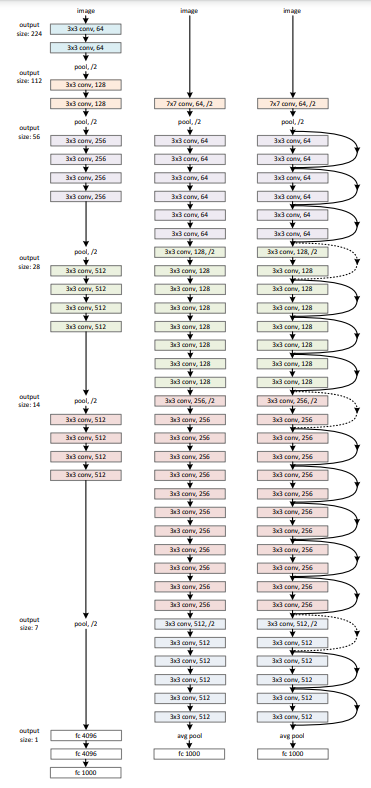
\includegraphics[width=0.5\linewidth]{ResNet}
\caption{ResNet structure compares to CNN and VGG structure \label{fig:resnet}}
\end{figure}

If the identity mapping can use the residual function to construct the next added layers, it means that the training loss will be less or equal to the previous shallower network. Hence if the next added layers can not be constructed by identity mapping, they will be skipped as the extra layers will not decrease the training loss. Figure \ref{fig:resnet} from the original paper clearly demonstrates the concepts \cite{Dummy:5}.

\subsubsection{EfficientNet}
\begin{figure}
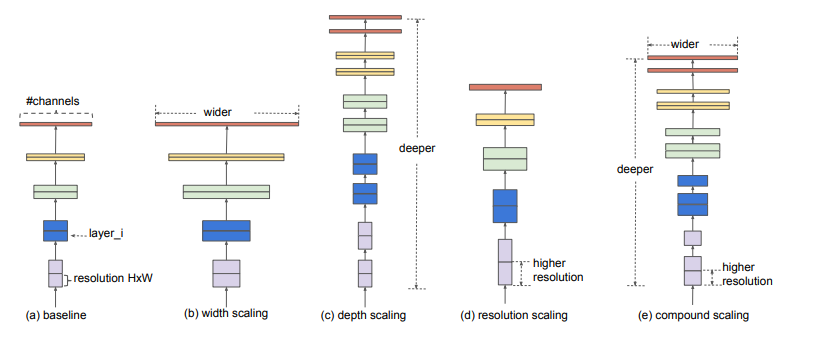
\includegraphics[width=\linewidth]{EffiNet}
\caption{EfficientNet structure compares to CNN and VGG structure \label{fig:efficientnet}}
\end{figure}

One of the latest neural network designed to improve accuracy by compound model scaling on a baseline model, i.e. finding the optimal width, depth and resolution of a network. Width refers to the number of filters in a conv layer, and depth refers to number of layers and resolution of image input \cite{Dummy:4} as is shown in figure \ref{fig:efficientnet}.

The paper found that scaling up any of the three would lead to better accuracy, however a complex model would receive diminishing benefit from further scaling, and balance of three dimensions is critical for finding the optimal structure that delivers better accuracy.

\subsubsection{LeNet}
\begin{figure}
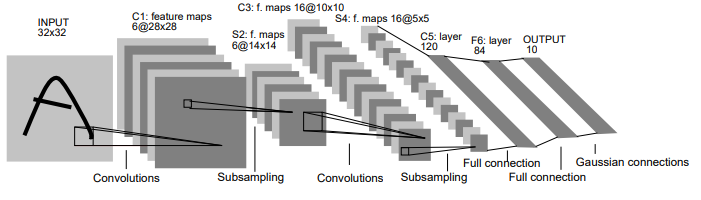
\includegraphics[width=\linewidth]{LeNet}
\caption{LeNet structure compares to CNN and VGG structure \label{fig:lenet}}
\end{figure}

Compared to other Networks, LeNet is rather straightforward. Through utilising a few convolution and subsampling layers as shown in figure 3, it can generate reasonable accuracy with a small dataset. In LeCun et al’s paper 60000 samples are used compared to ResNet of 1.28m samples. \cite{Dummy:7} The architecture is shown in figure \ref{fig:lenet}.

\subsection{Noise Transition Matrix}
Noise transition matrix is a novel solution to improve the accuracy of the classifier on a dataset with noisy label, i.e. incorrect label. The transition matrix is estimated through a set of (estimated) anchor points. Anchor points will have a probability close to one for one class, and close to zero for other classes. With the help of anchor points we can calculate the transition matrix as follows: \cite{Dummy:8}
\begin{equation}
P\left ( \tilde{Y} = j |\, X = x\right ) = \sum_{C}^{k=1}\, T_kj\, P\left ( Y = j |\, X = x\right ) = T_ij
\end{equation}

The two procedures can be used to reduce noise, with backward method being:
\begin{equation}
\left [ P\left ( Y = j |\, X\right ),...,P\left ( Y = C |\, X\right ) \right]^{T} = T^{-1}\,\left [ P\left ( \tilde{Y} = j |\, X\right ),...,P\left ( \tilde{Y} = C |\, X\right ) \right]^{T}
\end{equation}

The forward method estimates clean classification using:
\begin{equation}
\left [ P\left ( \tilde{Y} = j |\, X\right ),...,P\left ( \tilde{Y} = C |\, X\right ) \right]^{T} = T\,\left [ P\left ( Y = j |\, X\right ),...,P\left ( Y = C |\, X\right ) \right]^{T}
\end{equation}


\section{Methods}
\subsection{Label noise robust classification}
The noise transition matrix is implemented through both forward and backward methods. As well as using the transition matrix and anchor points, we implemented the loss correction approach demonstrated in Patrini et al's paper in our forward and backward procedure to enhance the performance of label noise reduction, as it agrees with the Noise Transition Matrix and Anchor point theory introduced in related work. Table \ref{tab:loss} shows the impact of forward loss and backward loss correction.

\begin{table}
\begin{tabular}{cccc}
loss & correction & $\mathbb{E}_{\boldsymbol{x},\tilde{\boldsymbol{y}}}$ & Hessian of $\mathbb{E}_{\boldsymbol{x},\tilde{\boldsymbol{y}}}$ \\\hline
$\ell$ & - & no guarantee & unchanged \\
$\ell^\leftarrow$ & $T^{-1}\cdot$ & unbiased estimator of $\ell$ & unchanged \\
$\ell^\rightarrow$ & $T\cdot$ & same minimizer of $\ell$ & no guarantee
\end{tabular}
\caption{Qualitative comparison of loss corrections. \label{tab:loss}}
\end{table}

\subsubsection{The backward correction procedure}
The classification for noisy data is calculated, the anchor points and hence the transition matrix can be estimated based upon the classifier result. The backward method estimates the clean data by the product of the inverse of transition matrix and transposed posterior probability.

\subsubsection{The forward correction procedure}
Forward method is implemented by first classifying the noisy data without noise reduction, by doing so we can estimate our anchor points, hence using the anchor points to estimate thee transition matrix. The probability of the clean data classification is estimated through maximizing the product of T and transposed posterior probability of the noisy data.

\subsection{Transition matrix estimation}
We can estimate each component of matrix $T$ just based on noisy class probability estimates. In particular, let $X^\prime$ be any set of feature vectors. This can be the training set itself, but not necessarily: we do not require this sample to have any label at all and therefore any unlabeled sample from the same distributions can be used as well. We can approximate $T$ with two steps: \cite{labelnoise}

\begin{equation}
\bar{\boldsymbol{x}}^i = \arg\max_{\boldsymbol{x}\in X^\prime} \hat{p}\left(\tilde{\boldsymbol{y}}=e^i|\boldsymbol{x}\right)
\label{eq:x}
\end{equation}

\begin{equation}
\hat{T}_{ij} = \hat{p}\left(\tilde{\boldsymbol{y}}=e^j|\bar{\boldsymbol{x}}^i\right)
\label{eq:T}
\end{equation}

\subsection{The overall algorithm}
Algorithm \ref{alg:training} shows how the forward and backward methods are implemented.

\begin{algorithm}
\begin{algorithmic}
\REQUIRE the noisy training set $S$, any loss $\ell$
\ENSURE $h\left(\cdot\right)$
\IF {$T$ is unknown}
  \STATE Train a classifier $\boldsymbol{h}\left(\boldsymbol{x}\right)$ on $S$ with loss $\ell$
  \STATE Obtain an unlabeled sample $X^\prime$
  \STATE Estimate $\hat{T}$ by Equations \eqref{eq:x}-\eqref{eq:T} on $X^\prime$
\ENDIF
\STATE Train the classifier $h\left(x\right)$ on $S$ with loss $\ell^\leftarrow$ or $\ell^\rightarrow$
\end{algorithmic}
\caption{Robust two-stage training \label{alg:training}}
\end{algorithm}

\section{Experiments}
\subsection{Datasets}
Three datasets were used in this experiment, each of which has 3 classes. For each dataset, the training and validation data contains label noise, whereas the test data is clean. Each dataset is scaled from the range $\left[0,255\right]$ to the range $\left[0,1\right]$, in order to improve the convergence and numerical stability. No other preprocessing is done, it is left to the algorithm in question to handle the feature engineering automatically. The experiment is performed 10 times with the training data separated into a random 80-20 train-validate split each time. The mean and standard deviation for each model across all trials is recorded. Table \ref{tab:dataset} provides the details of each dataset.

\begin{table}\begin{tabular}{ccccc} dataset & $n$ & $m$ & $\textup{shape}$ & $T$ \\\hline
FashionMNIST0.5 & 18000 & 3000 & (28 x 28) & $\begin{bmatrix}0.5 & 0.2 & 0.3\\0.3 & 0.5 & 0.2\\0.2 & 0.3 & 0.5\end{bmatrix}$\\
FashionMNIST0.6 & 18000 & 3000 & (28 x 28) & $\begin{bmatrix}0.4 & 0.3 & 0.3\\0.3 & 0.4 & 0.3\\0.3 & 0.3 & 0.4\end{bmatrix}$\\
CIFAR & 15000 & 3000 & (32 x 32 x 3) & $I$
\end{tabular}\caption{
  Datasets used in experiment, where $n$ is the number of training and validation examples, $m$ is the number of test examples, $\textup{shape}$ is the image shape and $T$ is the given transition matrix. For CIFAR the transition matrix is unknown. We substitute the identity matrix (i.e. assume no noise) as a point of reference.
  \label{tab:dataset}
}\end{table}

\subsubsection{Fashion MNIST 0.5}
FashionMNIST0.5 is a subset of the grayscale Fashion MNIST dataset originally based off the MNIST dataset of handwritten digits. It is commonly used as a baseline for evaluating machine learning algorithms. This particular dataset has had the labels randomly flipped according to Class-dependent label Noise (CCN), as indicated by the transition matrix in table \ref{tab:dataset}.

\subsubsection{Fashion MNIST 0.6}
FashionMNIST0.6 is a separate subset of the grayscale Fashion MNIST dataset. This particular dataset has had the labels randomly flipped according to Random Classification Noise (RCN), as indicated by the transition matrix in table \ref{tab:dataset}.

\subsubsection{CIFAR}
CIFAR is a subset of the RGB (color) CIFAR10 dataset commonly used to train machine learning algorithms. It has had the labels randomly flipped according to Class-dependent label Noise (CCN), however the transition matrix is unknown. For the sake of comparison, we include results on the identity matrix (assume no noise).

\subsection{Algorithms}
\subsubsection{Neural networks}
ResNet, EfficientNet, LeNet, a 1-layer net and a 3-layer net are implemented with both the forward and backward transition matrix methods. The implementation ensures the label noise robustness of the classifiers. The same optimization hyperparameters were used across all neural networks, as shown in table \ref{tab:nn}.

\begin{table}\begin{tabular}{cc} param & value\\\hline
optimizer & Adam\\
learning rate & 0.001\\
early stopping & validation loss\\
patience & 3\\
batch size & 1024\\
precision & 16-bit\\
hardware & AWS p3.2xlarge
\end{tabular}\caption{Parameters used for neural network training. \label{tab:nn}}\end{table}

\subsubsection{Black box classifiers}
The two black box algorithms are explored, LightGBM and logistic regression. Both classifiers' hyperparameters are tuned for each individual dataset as shown in table \ref{tab:lgb} and table \ref{tab:lr}.

We have no direct access to the gradient of these algorithms and instead treat them as black boxes. For this reason, only the backward method is applied to each classifier, as it requires no modification to the standard loss function (cross entropy).

\begin{table}\begin{tabular}{ccccccc} dataset & $\lambda_{\ell_1}$ & $\lambda_{\ell_2}$ & $n$ & $f$ & $b$ & $h$\\\hline
FashionMNIST0.5 & $10^{-4}$ & $10^{-4}$ & 9 & 95.20 & 94.78 & 1\\
FashionMNIST0.6 & 0 & 0 & 3 & 80.00 & 90.54 & 3\\
CIFAR & $10^{-5}$ & $10^{-2}$ & 8 & 100.00 & 97.15 & 3
\end{tabular}\caption{
  Hyperparameters used for LightGBM, where $\lambda_{\ell_1}$ is the $\ell_1$ regularization constant, $\lambda_{\ell_2}$ is the $\ell_2$ regularization constant, $n$ is number of leaves per tree, $f$ is feature fraction (\%), $b$ is bagging fraction (\%) and $h$ is bagging frequency.
  \label{tab:lgb}
}\end{table}

\begin{table}\begin{tabular}{cccc} dataset & $\lambda_{\ell_2}$ & solver & multiclass\\\hline
FashionMNIST0.5 & $10^{-3}$ & liblinear & ovr\\
FashionMNIST0.6 & $10^{-3}$ & saga & multinomial\\
CIFAR & $10^6$ & saga & ovr
\end{tabular}\caption{
  Hyperparameters used for logistic regression, where $\lambda_{\ell_2}$ is the $\ell_2$ regularization constant.
  \label{tab:lr}
}\end{table}

\subsection{Evaluation metrics}
\subsubsection{Top-1 Accuracy}
The performance of each classifier is evaluated with the top-1 accuracy metric, that is,

\begin{equation}
\textup{top-1 accuracy} = \frac{\textup{number of correctly classified examples}}{\textup{total number of test examples}}
\end{equation}

\subsubsection{Relative Reconstruction Errors (RRE)}
In order to validate the effectiveness of the transition matrix estimation, we calculate the Relative Reconstruction Errors:

\begin{equation}
\textup{RRE} = \frac{\left\|T - \hat{T}\right\|_F}{\left\|T\right\|_F}
\end{equation}

where $T$ is the given transition matrix and $\hat{T}$ is the estimated transition matrix.


\subsection{Results}
\subsubsection{Test accuracy using given transition matrices}
Figures \ref{fig:acc-FashionMNIST0.5} and \ref{fig:acc-FashionMNIST0.6} show LeNet, 1-layer, 3-layer and LightGBM performing reasonably well. For the neural networks, the forward method consistently outperforms the backward method. Figure \ref{fig:acc-CIFAR} shows results using the identity transition matrix (i.e. assuming no noise), and the results are consistent with the first two datasets. This suggests that the robustness of the underlying classifier is important to achieving high accuracy.

\begin{figure}\begin{tikzpicture}\begin{axis}[
    title={FashionMNIST0.5 - given},
    ybar, nodes near coords,
    xlabel={Model},
    xtick=data,
    xticklabels from table={\resultsa}{model},
    x tick label style={rotate=90,anchor=east},
    ylabel={Top-1 Accuracy (\%)},
]\addplot table[x expr=\coordindex, y expr=100*\thisrow{acc}]{\resultsa};\end{axis}\end{tikzpicture}\caption{
  Top-1 accuracy on the FashionMNIST0.5 test set using the given transition matrix.
  \label{fig:acc-FashionMNIST0.5}
}\end{figure}

\begin{figure}\begin{tikzpicture}\begin{axis}[
    title={FashionMNIST0.6 - given},
    ybar, nodes near coords,
    xlabel={Model},
    xtick=data,
    xticklabels from table={\resultsb}{model},
    x tick label style={rotate=90,anchor=east},
    ylabel={Top-1 Accuracy (\%)},
]\addplot table[x expr=\coordindex, y expr=100*\thisrow{acc}]{\resultsb};\end{axis}\end{tikzpicture}\caption{
  Top-1 accuracy on the FashionMNIST0.6 test set using the given transition matrix.
  \label{fig:acc-FashionMNIST0.6}
}\end{figure}

\begin{figure}\begin{tikzpicture}\begin{axis}[
    title={CIFAR - given},
    ybar, nodes near coords,
    xlabel={Model},
    xtick=data,
    xticklabels from table={\resultsc}{model},
    x tick label style={rotate=90,anchor=east},
    ylabel={Top-1 Accuracy (\%)},
]\addplot table[x expr=\coordindex, y expr=100*\thisrow{acc}]{\resultsc};\end{axis}\end{tikzpicture}\caption{
  Top-1 accuracy on the CIFAR test set using the given transition matrix.
  \label{fig:acc-CIFAR}
}\end{figure}

\subsubsection{Test accuracy using estimated transition matrices}
Figures \ref{fig:acc-hat-FashionMNIST0.5} and \ref{fig:acc-hat-FashionMNIST0.6} show consistent performance compared to the results on the given transition matrices. LightGBM performs paticularly well on the first two datasets using the estimated transition matrix. Figure \ref{fig:acc-hat-CIFAR} shows consistently better results than when assuming no noise.

\begin{figure}\begin{tikzpicture}\begin{axis}[
    title={FashionMNIST0.5 - estimated},
    ybar, nodes near coords,
    xlabel={Model},
    xtick=data,
    xticklabels from table={\resultsa}{model},
    x tick label style={rotate=90,anchor=east},
    ylabel={Top-1 Accuracy (\%)},
]\addplot table[x expr=\coordindex, y expr=100*\thisrow{acc-hat}]{\resultsa};\end{axis}\end{tikzpicture}\caption{
  Top-1 accuracy on the FashionMNIST0.5 test set using the estimated transition matrix.
  \label{fig:acc-hat-FashionMNIST0.5}
}\end{figure}

\begin{figure}\begin{tikzpicture}\begin{axis}[
    title={FashionMNIST0.6 - estimated},
    ybar, nodes near coords,
    xlabel={Model},
    xtick=data,
    xticklabels from table={\resultsb}{model},
    x tick label style={rotate=90,anchor=east},
    ylabel={Top-1 Accuracy (\%)},
]\addplot table[x expr=\coordindex, y expr=100*\thisrow{acc-hat}]{\resultsb};\end{axis}\end{tikzpicture}\caption{
  Top-1 accuracy on the FashionMNIST0.6 test set using the estimated transition matrix.
  \label{fig:acc-hat-FashionMNIST0.6}
}\end{figure}

\begin{figure}\begin{tikzpicture}\begin{axis}[
    title={CIFAR - estimated},
    ybar, nodes near coords,
    xlabel={Model},
    xtick=data,
    xticklabels from table={\resultsc}{model},
    x tick label style={rotate=90,anchor=east},
    ylabel={Top-1 Accuracy (\%)},
]\addplot table[x expr=\coordindex, y expr=100*\thisrow{acc-hat}]{\resultsc};\end{axis}\end{tikzpicture}\caption{
  Top-1 accuracy on the CIFAR test set using the estimated transition matrix.
  \label{fig:acc-hat-FashionMNIST0.6}
}\end{figure}


\subsubsection{RRE of estimated transition matrices}
Figures \ref{fig:T-hat-RRE-FashionMNIST0.5} and \ref{fig:T-hat-RRE-FashionMNIST0.6} show LeNet and LightGBM to be accurately estimating the transition matrix, which explains their higher levels of accuracy. Figure \ref{fig:T-hat-RRE-CIFAR} shows that EfficientNet and logistic regression are underfitting the transition matrix (they are predicting close to identity matrix). Perhaps the EfficientNet training is stopping too early due to poor generalization on the validation set.

\begin{figure}\begin{tikzpicture}\begin{axis}[
    title={FashionMNIST0.5 - RRE},
    ybar, nodes near coords,
    xlabel={Model},
    xtick=data,
    xticklabels from table={\resultsa}{model},
    x tick label style={rotate=90,anchor=east},
    ylabel={RRE},
]\addplot table[x expr=\coordindex, y expr=\thisrow{T-hat-RRE}]{\resultsa};\end{axis}\end{tikzpicture}\caption{
  Relative Reconstruction Errors on the FashionMNIST0.5 transition matrix.
  \label{fig:T-hat-RRE-FashionMNIST0.5}
}\end{figure}

\begin{figure}\begin{tikzpicture}\begin{axis}[
    title={FashionMNIST0.6 - RRE},
    ybar, nodes near coords,
    xlabel={Model},
    xtick=data,
    xticklabels from table={\resultsb}{model},
    x tick label style={rotate=90,anchor=east},
    ylabel={RRE},
]\addplot table[x expr=\coordindex, y expr=\thisrow{T-hat-RRE}]{\resultsb};\end{axis}\end{tikzpicture}\caption{
  Relative Reconstruction Errors on the FashionMNIST0.6 transition matrix.
  \label{fig:T-hat-RRE-FashionMNIST0.6}
}\end{figure}

\begin{figure}\begin{tikzpicture}\begin{axis}[
    title={CIFAR - RRE},
    ybar, nodes near coords,
    xlabel={Model},
    xtick=data,
    xticklabels from table={\resultsc}{model},
    x tick label style={rotate=90,anchor=east},
    ylabel={RRE},
]\addplot table[x expr=\coordindex, y expr=\thisrow{T-hat-RRE}]{\resultsc};\end{axis}\end{tikzpicture}\caption{
  Relative Reconstruction Errors on the CIFAR transition matrix.
  \label{fig:T-hat-RRE-CIFAR}
}\end{figure}

\subsubsection{Estimated transition matrices}
Tables \ref{tab:T-FashionMNIST0.5} and \ref{tab:T-FashionMNIST0.6} list the estimated transition matrices on the first two datasets. From the results we can see that LeNet and LightGBM have the lowest error on the first two respective datasets. Table \ref{tab:T-CIFAR} lists the estimated transition matrices on the CIFAR dataset. Based on the RRE results from the first two datasets and the accuracy results, we believe either LeNet or LightGBM to be generating the most accurate transition matrix for the CIFAR dataset.

\begin{table}\begin{tabular}{ccc}Model&T&STD\\\hline
lenet & $\begin{bmatrix}0.6088 & 0.1533 & 0.2544\\0.2667 & 0.5980 & 0.1733\\0.1246 & 0.2488 & 0.5723\end{bmatrix}$ & $\begin{bmatrix}0.0308 & 0.0153 & 0.0235\\0.0239 & 0.0425 & 0.0240\\0.0243 & 0.0328 & 0.0417\end{bmatrix}$\\
lenet-backward & $\begin{bmatrix}0.6001 & 0.1512 & 0.2485\\0.2654 & 0.5968 & 0.1678\\0.1346 & 0.2520 & 0.5838\end{bmatrix}$ & $\begin{bmatrix}0.0183 & 0.0160 & 0.0203\\0.0213 & 0.0335 & 0.0239\\0.0156 & 0.0361 & 0.0393\end{bmatrix}$\\
linear & $\begin{bmatrix}0.6861 & 0.1675 & 0.2229\\0.2084 & 0.7866 & 0.1491\\0.1055 & 0.0459 & 0.6280\end{bmatrix}$ & $\begin{bmatrix}0.0623 & 0.0277 & 0.0175\\0.0413 & 0.0300 & 0.0185\\0.0285 & 0.0040 & 0.0179\end{bmatrix}$\\
linear-backward & $\begin{bmatrix}0.6771 & 0.1866 & 0.2346\\0.2040 & 0.7717 & 0.1493\\0.1189 & 0.0417 & 0.6160\end{bmatrix}$ & $\begin{bmatrix}0.0471 & 0.0321 & 0.0172\\0.0313 & 0.0366 & 0.0152\\0.0323 & 0.0088 & 0.0174\end{bmatrix}$\\
threelayer & $\begin{bmatrix}0.6623 & 0.2270 & 0.2306\\0.2312 & 0.6642 & 0.1388\\0.1065 & 0.1088 & 0.6306\end{bmatrix}$ & $\begin{bmatrix}0.0646 & 0.0598 & 0.0466\\0.0525 & 0.0640 & 0.0245\\0.0221 & 0.0838 & 0.0573\end{bmatrix}$\\
threelayer-backward & $\begin{bmatrix}0.6520 & 0.2012 & 0.2115\\0.2502 & 0.6631 & 0.1433\\0.0978 & 0.1357 & 0.6451\end{bmatrix}$ & $\begin{bmatrix}0.0590 & 0.0490 & 0.0416\\0.0423 & 0.0592 & 0.0261\\0.0266 & 0.0809 & 0.0573\end{bmatrix}$\\
resnet & $\begin{bmatrix}0.6987 & 0.1469 & 0.2299\\0.1788 & 0.7097 & 0.1542\\0.1224 & 0.1433 & 0.6159\end{bmatrix}$ & $\begin{bmatrix}0.0410 & 0.0690 & 0.0343\\0.0376 & 0.1009 & 0.0325\\0.0318 & 0.0520 & 0.0357\end{bmatrix}$\\
resnet-backward & $\begin{bmatrix}0.7232 & 0.1435 & 0.2060\\0.1645 & 0.6737 & 0.1280\\0.1123 & 0.1828 & 0.6660\end{bmatrix}$ & $\begin{bmatrix}0.0777 & 0.0451 & 0.0388\\0.0558 & 0.0514 & 0.0307\\0.0384 & 0.0229 & 0.0517\end{bmatrix}$\\
efficientnet & $\begin{bmatrix}0.9885 & 0.0062 & 0.0210\\0.0078 & 0.9825 & 0.0260\\0.0037 & 0.0113 & 0.9530\end{bmatrix}$ & $\begin{bmatrix}0.0272 & 0.0139 & 0.0365\\0.0206 & 0.0470 & 0.0479\\0.0074 & 0.0335 & 0.0840\end{bmatrix}$\\
efficientnet-backward & $\begin{bmatrix}0.9609 & 0.0304 & 0.0198\\0.0246 & 0.9357 & 0.0162\\0.0145 & 0.0338 & 0.9640\end{bmatrix}$ & $\begin{bmatrix}0.0657 & 0.0445 & 0.0404\\0.0434 & 0.0829 & 0.0270\\0.0228 & 0.0443 & 0.0627\end{bmatrix}$\\
lgb & $\begin{bmatrix}0.6343 & 0.1457 & 0.1949\\0.2239 & 0.6608 & 0.1598\\0.1418 & 0.1935 & 0.6452\end{bmatrix}$ & $\begin{bmatrix}0.0000 & 0.0000 & 0.0000\\0.0000 & 0.0000 & 0.0000\\0.0000 & 0.0000 & 0.0000\end{bmatrix}$\\
logistic & $\begin{bmatrix}0.9954 & 0.0014 & 0.0145\\0.0002 & 0.9965 & 0.0454\\0.0043 & 0.0020 & 0.9400\end{bmatrix}$ & $\begin{bmatrix}0.0000 & 0.0000 & 0.0000\\0.0000 & 0.0000 & 0.0000\\0.0000 & 0.0000 & 0.0000\end{bmatrix}$\\
\end{tabular}\caption{
  Estimated transition matrix mean and standard deviation on FashionMNIST0.5 dataset.
  \label{tab:T-FashionMNIST0.5}
}\end{table}
\begin{table}\begin{tabular}{ccc}Model&T&STD\\\hline
lenet & $\begin{bmatrix}0.5923 & 0.2982 & 0.2276\\0.2421 & 0.4525 & 0.2834\\0.1655 & 0.2494 & 0.4890\end{bmatrix}$ & $\begin{bmatrix}0.0334 & 0.0138 & 0.0192\\0.0118 & 0.0133 & 0.0125\\0.0237 & 0.0118 & 0.0119\end{bmatrix}$\\
lenet-backward & $\begin{bmatrix}0.5515 & 0.2993 & 0.2365\\0.2541 & 0.4439 & 0.2823\\0.1944 & 0.2568 & 0.4812\end{bmatrix}$ & $\begin{bmatrix}0.0367 & 0.0123 & 0.0190\\0.0118 & 0.0164 & 0.0084\\0.0282 & 0.0131 & 0.0235\end{bmatrix}$\\
linear & $\begin{bmatrix}0.7112 & 0.2676 & 0.2523\\0.1280 & 0.4910 & 0.2114\\0.1608 & 0.2413 & 0.5363\end{bmatrix}$ & $\begin{bmatrix}0.0486 & 0.0370 & 0.0157\\0.0174 & 0.0538 & 0.0200\\0.0349 & 0.0348 & 0.0229\end{bmatrix}$\\
linear-backward & $\begin{bmatrix}0.7178 & 0.2942 & 0.2470\\0.1223 & 0.4765 & 0.2159\\0.1599 & 0.2293 & 0.5371\end{bmatrix}$ & $\begin{bmatrix}0.0492 & 0.0285 & 0.0322\\0.0201 & 0.0356 & 0.0318\\0.0336 & 0.0338 & 0.0223\end{bmatrix}$\\
threelayer & $\begin{bmatrix}0.6308 & 0.2836 & 0.2554\\0.2033 & 0.4622 & 0.2556\\0.1659 & 0.2542 & 0.4891\end{bmatrix}$ & $\begin{bmatrix}0.0644 & 0.0171 & 0.0182\\0.0346 & 0.0386 & 0.0222\\0.0351 & 0.0315 & 0.0385\end{bmatrix}$\\
threelayer-backward & $\begin{bmatrix}0.5952 & 0.2961 & 0.2566\\0.2212 & 0.4602 & 0.2654\\0.1836 & 0.2436 & 0.4781\end{bmatrix}$ & $\begin{bmatrix}0.0571 & 0.0140 & 0.0101\\0.0312 & 0.0243 & 0.0093\\0.0296 & 0.0285 & 0.0146\end{bmatrix}$\\
resnet & $\begin{bmatrix}0.6556 & 0.2749 & 0.1997\\0.1837 & 0.5254 & 0.1958\\0.1608 & 0.1997 & 0.6045\end{bmatrix}$ & $\begin{bmatrix}0.0841 & 0.0455 & 0.0501\\0.0525 & 0.0622 & 0.0456\\0.0557 & 0.0527 & 0.0718\end{bmatrix}$\\
resnet-backward & $\begin{bmatrix}0.6291 & 0.3154 & 0.2559\\0.1868 & 0.4611 & 0.2295\\0.1842 & 0.2235 & 0.5146\end{bmatrix}$ & $\begin{bmatrix}0.0942 & 0.0468 & 0.0330\\0.0464 & 0.0548 & 0.0184\\0.0506 & 0.0412 & 0.0387\end{bmatrix}$\\
efficientnet & $\begin{bmatrix}0.9654 & 0.0321 & 0.0209\\0.0158 & 0.9413 & 0.0184\\0.0188 & 0.0266 & 0.9607\end{bmatrix}$ & $\begin{bmatrix}0.0531 & 0.0668 & 0.0378\\0.0258 & 0.0941 & 0.0256\\0.0285 & 0.0392 & 0.0622\end{bmatrix}$\\
efficientnet-backward & $\begin{bmatrix}0.9950 & 0.0087 & 0.0039\\0.0016 & 0.9775 & 0.0026\\0.0035 & 0.0138 & 0.9935\end{bmatrix}$ & $\begin{bmatrix}0.0105 & 0.0135 & 0.0116\\0.0044 & 0.0359 & 0.0076\\0.0064 & 0.0226 & 0.0192\end{bmatrix}$\\
lgb & $\begin{bmatrix}0.4306 & 0.2876 & 0.2921\\0.2879 & 0.4202 & 0.2865\\0.2815 & 0.2921 & 0.4214\end{bmatrix}$ & $\begin{bmatrix}0.0000 & 0.0000 & 0.0000\\0.0000 & 0.0000 & 0.0000\\0.0000 & 0.0000 & 0.0000\end{bmatrix}$\\
logistic & $\begin{bmatrix}0.9525 & 0.0587 & 0.0322\\0.0127 & 0.9136 & 0.0173\\0.0348 & 0.0277 & 0.9505\end{bmatrix}$ & $\begin{bmatrix}0.0004 & 0.0002 & 0.0004\\0.0001 & 0.0003 & 0.0002\\0.0003 & 0.0001 & 0.0006\end{bmatrix}$\\
\end{tabular}\caption{
  Estimated transition matrix mean and standard deviation on FashionMNIST0.6 dataset.
  \label{tab:T-FashionMNIST0.6}
}\end{table}
\begin{table}\begin{tabular}{ccc}Model&T&STD\\\hline
lenet & $\begin{bmatrix}0.4388 & 0.2145 & 0.2343\\0.2931 & 0.5167 & 0.2615\\0.2681 & 0.2688 & 0.5042\end{bmatrix}$ & $\begin{bmatrix}0.0270 & 0.0346 & 0.0469\\0.0270 & 0.0271 & 0.0322\\0.0186 & 0.0229 & 0.0387\end{bmatrix}$\\
lenet-backward & $\begin{bmatrix}0.4409 & 0.1942 & 0.2434\\0.2814 & 0.5338 & 0.2652\\0.2777 & 0.2721 & 0.4915\end{bmatrix}$ & $\begin{bmatrix}0.0370 & 0.0504 & 0.0350\\0.0398 & 0.0276 & 0.0358\\0.0410 & 0.0392 & 0.0274\end{bmatrix}$\\
linear & $\begin{bmatrix}0.4999 & 0.2329 & 0.2158\\0.2918 & 0.5095 & 0.2318\\0.2083 & 0.2576 & 0.5524\end{bmatrix}$ & $\begin{bmatrix}0.0314 & 0.0201 & 0.0308\\0.0309 & 0.0232 & 0.0291\\0.0522 & 0.0236 & 0.0207\end{bmatrix}$\\
linear-backward & $\begin{bmatrix}0.5069 & 0.2471 & 0.2275\\0.2796 & 0.5060 & 0.2205\\0.2135 & 0.2469 & 0.5520\end{bmatrix}$ & $\begin{bmatrix}0.0268 & 0.0109 & 0.0184\\0.0377 & 0.0264 & 0.0201\\0.0473 & 0.0222 & 0.0161\end{bmatrix}$\\
threelayer & $\begin{bmatrix}0.4551 & 0.2554 & 0.2071\\0.3149 & 0.4607 & 0.2727\\0.2300 & 0.2839 & 0.5202\end{bmatrix}$ & $\begin{bmatrix}0.0395 & 0.0322 & 0.0446\\0.0438 & 0.0267 & 0.0422\\0.0644 & 0.0278 & 0.0652\end{bmatrix}$\\
threelayer-backward & $\begin{bmatrix}0.4445 & 0.2898 & 0.2353\\0.3390 & 0.4376 & 0.2465\\0.2165 & 0.2726 & 0.5182\end{bmatrix}$ & $\begin{bmatrix}0.0290 & 0.0300 & 0.0274\\0.0419 & 0.0249 & 0.0222\\0.0468 & 0.0291 & 0.0334\end{bmatrix}$\\
resnet & $\begin{bmatrix}0.6655 & 0.1463 & 0.1525\\0.1346 & 0.6494 & 0.1502\\0.1999 & 0.2043 & 0.6973\end{bmatrix}$ & $\begin{bmatrix}0.1765 & 0.0831 & 0.0961\\0.0993 & 0.1189 & 0.1023\\0.1176 & 0.0980 & 0.1404\end{bmatrix}$\\
resnet-backward & $\begin{bmatrix}0.7334 & 0.1632 & 0.1519\\0.1153 & 0.6529 & 0.1157\\0.1513 & 0.1839 & 0.7324\end{bmatrix}$ & $\begin{bmatrix}0.1893 & 0.0826 & 0.0895\\0.1101 & 0.1726 & 0.1002\\0.0915 & 0.1061 & 0.1696\end{bmatrix}$\\
efficientnet & $\begin{bmatrix}0.8577 & 0.0930 & 0.0811\\0.0532 & 0.8075 & 0.0670\\0.0891 & 0.0995 & 0.8520\end{bmatrix}$ & $\begin{bmatrix}0.2459 & 0.1280 & 0.1299\\0.0949 & 0.2710 & 0.1100\\0.1530 & 0.1520 & 0.2227\end{bmatrix}$\\
efficientnet-backward & $\begin{bmatrix}0.6847 & 0.1709 & 0.1268\\0.1309 & 0.6172 & 0.1426\\0.1844 & 0.2119 & 0.7305\end{bmatrix}$ & $\begin{bmatrix}0.2765 & 0.1482 & 0.1270\\0.1126 & 0.3184 & 0.1558\\0.1788 & 0.1816 & 0.2600\end{bmatrix}$\\
lgb & $\begin{bmatrix}0.4649 & 0.2344 & 0.2378\\0.2924 & 0.5035 & 0.2666\\0.2427 & 0.2621 & 0.4956\end{bmatrix}$ & $\begin{bmatrix}0.0000 & 0.0000 & 0.0000\\0.0000 & 0.0000 & 0.0000\\0.0000 & 0.0000 & 0.0000\end{bmatrix}$\\
logistic & $\begin{bmatrix}0.7887 & 0.1280 & 0.1201\\0.1641 & 0.7512 & 0.1001\\0.0472 & 0.1209 & 0.7798\end{bmatrix}$ & $\begin{bmatrix}0.0005 & 0.0120 & 0.0005\\0.0005 & 0.0004 & 0.0006\\0.0002 & 0.0119 & 0.0005\end{bmatrix}$\\
\end{tabular}\caption{
  Estimated transition matrix mean and standard deviation on CIFAR dataset.
  \label{tab:T-CIFAR}
}\end{table}


\subsection{Discussion}
\begin{table}\pgfplotstabletypeset[
    columns={model,acc,acc-std,acc-hat,acc-hat-std,T-hat-RRE,T-hat-RRE-std},
    columns/model/.style={string type,column name=Model},
    columns/acc/.style={multiply by=100,column name={Acc\% given}},
    columns/acc-std/.style={multiply by=100,column name={STD}},
    columns/acc-hat/.style={multiply by=100,column name={Acc\% estimated}},
    columns/acc-hat-std/.style={multiply by=100,column name={STD}},
    columns/T-hat-RRE/.style={column name={RRE}},
    columns/T-hat-RRE-std/.style={column name={STD}},
    every head row/.style={after row=\hline},
]{\resultsa}\caption{
  FashionMNIST0.5 top-1 accuracy mean and standard deviation on given and estimated transition matrices respectively, and estimated transition matrix Relative Reconstruction Errors (RRE).
  \label{tab:FashionMNIST0.5}
}\end{table}
\begin{table}\pgfplotstabletypeset[
    columns={model,acc,acc-std,acc-hat,acc-hat-std,T-hat-RRE,T-hat-RRE-std},
    columns/model/.style={string type,column name=Model},
    columns/acc/.style={multiply by=100,column name={Acc\% given}},
    columns/acc-std/.style={multiply by=100,column name={STD}},
    columns/acc-hat/.style={multiply by=100,column name={Acc\% estimated}},
    columns/acc-hat-std/.style={multiply by=100,column name={STD}},
    columns/T-hat-RRE/.style={column name={RRE}},
    columns/T-hat-RRE-std/.style={column name={STD}},
    every head row/.style={after row=\hline},
]{\resultsb}\caption{
  FashionMNIST0.6 top-1 accuracy mean and standard deviation on given and estimated transition matrices respectively, and estimated transition matrix Relative Reconstruction Errors (RRE).
  \label{tab:FashionMNIST0.6}
}\end{table}
\begin{table}\pgfplotstabletypeset[
    columns={model,acc,acc-std,acc-hat,acc-hat-std,T-hat-RRE,T-hat-RRE-std},
    columns/model/.style={string type,column name=Model},
    columns/acc/.style={multiply by=100,column name={Acc\% given}},
    columns/acc-std/.style={multiply by=100,column name={STD}},
    columns/acc-hat/.style={multiply by=100,column name={Acc\% estimated}},
    columns/acc-hat-std/.style={multiply by=100,column name={STD}},
    columns/T-hat-RRE/.style={column name={RRE}},
    columns/T-hat-RRE-std/.style={column name={STD}},
    every head row/.style={after row=\hline},
]{\resultsc}\caption{
  CIFAR top-1 accuracy mean and standard deviation on given and estimated transition matrices respectively, and estimated transition matrix Relative Reconstruction Errors (RRE).
  \label{tab:CIFAR}
}\end{table}

As we can see in tables \ref{tab:FashionMNIST0.5} and \ref{tab:FashionMNIST0.6}, LightGBM performed very well with FashionMNIST datasets compared to other networks, mainly due to two factors. Firstly the FashionMNIST datasets have a relatively low dimension and features, LightGBM is able to learn through information gain, secondly, due to the small sample size of the dataset, some of the complex networks are not able to unleash their full potential. This is especially true when the data contains noisy label, as small dataset limits the ability of complex neural network to give an accurate prediction on the noisy dataset, hence the estimated transition matrix is likely to contain error. The poorly calculated transition matrix is inadequate to reduce the noise in the noisy label, which would ultimately lead to a poor result in predicting the true class of the given data. The results show that neural network only have a marginal increase in accuracy.

However, when the dataset becomes larger and more complex, i.e. more features and increased dimensions, the classification accuracy of neural network starts to surpass the baseline LightGBM model, as can be seen in table \ref{tab:CIFAR}. It is because that LightGBM is unable to fully and appropriately learn the increasing complex features. Deep neural networks have the capability of learning complex features through a large number of filters where each feature can be extracted and assigned the appropriate weight. The results confirm the theory as neural networks outperform LightGBM on the more complex CIFAR dataset.

The advantage of simple network when working on small dataset is shown again through high performance of LeNet. ResNet and EfficientNet are two very well-designed networks however, in our experiment due to lack of data, their complexity means that they require a large amount of data to avoid high bias (underfitting) and high variance (overfitting).


\section{Conclusion}
Overall, the experiment can demonstrate the increase in robustness by using transition matrix. The limitations of each classifier are explored. LightGBM being able to learn well in simple dataset, however, struggles when dataset becomes more complex. Neural networks in general suffers from limited data sample size, and we see simple structure such as LeNet excels when sample size is small. The accuracy of the classifier has a significant impact on its robustness, as anchor point is used. Hence to accurately predict the true class using a noisy labeled dataset would largely depend on the learning ability of the classifier.

\subsection{Future work}
Using transition matrix is an effective way to increase the robustness of a classifier, however, it does create a dependency on the classifier’s accuracy. This generally will not be an issue when a large dataset is available, however when the data is limited, it might be useful to reduce the dependence on classifier's accuracy.


\pagebreak\printbibliography\appendix

\section{Running the code}
The experiment code is contained in a single file \texttt{algorithm.py}, which can either be imported as a module or run as a standalone script.

\begin{itemize}
\item Dependencies: \texttt{pip install jsonlines lightgbm optuna pytorch-lightning}
\item Usage: \texttt{./algorithm/algorithm.py >results.csv 2>algorithm.log}
\item Hyperparam tuning: \texttt{./algorithm/algorithm.py -t >tuning\_results.jsonl 2>tuning.log}
\item Generate latex tables: \texttt{./algorithm/algorithm.py -l <results.csv}
\item Help: \texttt{./algorithm/algorithm.py -h}
\end{itemize}

The code can be configured (number of trials, GPU settings, batch size, etc) via hard-coded constants at the top of the file. At the bottom of the file, there is an additional \texttt{TRAINING\_CONFIG} constant which controls which (model, dataset) combinations to run in the evaluation. Entries can be rearranged and/or commented out if desired.

\end{document}
